\documentclass[11pt,a4paper, uplatex]{jsreport}
%
\usepackage{amsmath,amssymb}
\usepackage{bm}
\usepackage[dvipdfmx]{graphicx}
\usepackage{ascmac}
\usepackage{listings,jlisting}
\usepackage{underscore}
\usepackage{url}
\usepackage{subfig}
\usepackage[]{mcode}
\lstset{
    frame=single,
    numbers=left,
    tabsize=2
}
\lstset{language=Matlab,%
    %basicstyle=\color{red},
    breaklines=true,%
    morekeywords={matlab2tikz},
    keywordstyle=\color{blue},%
    morekeywords=[2]{1}, keywordstyle=[2]{\color{black}},
    identifierstyle=\color{black},%
    showstringspaces=false,%without this there will be a symbol in the places where there is a space
    numbers=left,%
    numberstyle={\tiny \color{black}},% size of the numbers
    numbersep=9pt, % this defines how far the numbers are from the text
    emph=[1]{for,end,break},emphstyle=[1]\color{red}, %some words to emphasise
    %emph=[2]{word1,word2}, emphstyle=[2]{style},
}
%
\setlength{\textwidth}{\fullwidth}
\setlength{\textheight}{40\baselineskip}
\addtolength{\textheight}{\topskip}
\setlength{\voffset}{-0.2in}
\setlength{\topmargin}{0pt}
\setlength{\headheight}{0pt}
\setlength{\headsep}{0pt}
%
\newcommand{\divergence}{\mathrm{div}\,}  %ダイバージェンス
\newcommand{\grad}{\mathrm{grad}\,}  %グラディエント
\newcommand{\rot}{\mathrm{rot}\,}  %ローテーション
%
\title{Web画像を用いた物体認識実験}
\author{1510151  栁 裕太}
\date{\today}
\pagestyle{empty}
\begin{document}
\maketitle
\thispagestyle{empty}
\tableofcontents
\chapter{2クラス物体分類実験}
\section{課題内容}
異なる2クラス各200枚の画像データセットをそれぞれポジティブ画像・ネガティブ画像として分類し、
それらを対象に2クラス画像分類を行った。
今回対象としてのは以下のパターンである。
\begin{itemize}
  \item ポジティブ: タスマニアデビル
  \item ネガティブ: カピバラ
\end{itemize}
\begin{itemize}
  \item ポジティブ: タスマニアデビル
  \item ネガティブ: それ以外
\end{itemize}
なお"それ以外"とは、\texttt{/usr/local/class/object/bgimg}
に存在する900枚の画像から無作為に選出した600枚(ポジティブ画像数の3倍)のことを指す。

分類は以下の3種類の方法を行い、分類精度の比較を行った。
\begin{itemize}
  \item カラーヒストグラムと最近傍分類
  \item BoFベクトルと非線形SVMによる分類
  \item MatConvnetの標準ネットワーク(AlexNet)による DCNN特徴量と線形SVM
\end{itemize}

なお、評価は5-fold cross validation方式を採用した。

\section{設計方針}
\subsection{画像収集方法}\label{sec:collectimg}
実験に先立ち、画像の収集を行った。
Flickerから画像を収集し、横幅320pxにリサイズされた画像へのURLを表示するサイト
(https://goo.gl/v8wbsR)を使用した。
検索ワードは
\begin{itemize}
  \item タスマニアデビル: Tasmanian Devil
  \item カピバラ: Capybara
\end{itemize}
とした。得られた300枚の画像から明らかに当該動物が映っていない画像をここから除外し、
さらに全体の画像が200枚になるように調整した。
\subsection{codebook/filelist作成}\label{sec:mkCdBookFlist}
予め、後の処理で使用する全ポジティブ・ネガティブ画像のSIFT特徴が記されたコードブックを作成した。
また同時に分析対象のファイルのpathが記されたfilelistも作成した。
該当スクリプトと出力結果ファイルは
\begin{itemize}
  \item タスマニアデビル/カピバラ(以下、t/cと表記)
  \begin{itemize}
    \item codebook: \texttt{mk_codebook_tc.m} → \texttt{codebook-tc.mat}
    \item filelist: \texttt{flist_tc.m} → \texttt{filelist-tc.mat}
  \end{itemize}
  \item タスマニアデビル/それ以外(以下、otherと表記)
  \begin{itemize}
    \item codebook: \texttt{mk_codebook_other.m} → \texttt{codebook-other.mat}
    \item filelist: \texttt{flist_other.m} → \texttt{filelist-other.mat}
  \end{itemize}
\end{itemize}
である。
\subsection{カラーヒストグラムと最近傍分類}\label{sec:defhist}
評価を行う\texttt{capybara_hist.m}(カピバラ相手)と\texttt{others_hist.m}(それ以外相手)、
2者に共通して画像のカラーヒストグラムを返す関数\texttt{mk_hist.m}の2ファイルを作成した。
最終的にどれだけの割合で正しくクラス分類できたか確率を返すようになっている。
\subsection{BoFベクトルと非線形SVMによる分類}\label{sec:defbof}
評価を行う部分と、入力された\texttt{filelist}記載の画像をBoFベクトル化して返す部分を関数として実装した。
該当するスクリプト・出力結果ファイルは以下の通りである。
\begin{itemize}
  \item t/c
  \begin{itemize}
    \item 評価: \texttt{bof_svm_tc.m}
    \item BoF化: \texttt{mk_svm_tc.m} → \texttt{all_bovw-tc.mat}
  \end{itemize}
  \item other
  \begin{itemize}
    \item 評価: \texttt{bof_svm_others.m}
    \item BoF化: \texttt{mk_svm_others.m} → \texttt{all_bovw-others.mat}
  \end{itemize}
\end{itemize}
最終的にどれだけの割合で正しくクラス分類できたか確率を返すようにした。
\subsection{MatConvnetの標準ネットワークによる DCNN特徴量と線形SVM}\label{sec:defdcnn}
評価を行う部分と、入力された\texttt{filelist}記載の画像のDCNN特徴量を返す部分を関数として実装した。
該当するスクリプト・出力結果ファイルは以下の通りである。
\begin{itemize}
  \item t/c
  \begin{itemize}
    \item 評価: \texttt{dcnn_svm_tc.m}
    \item DCNN: \texttt{mk_dcnnlist.m} → \texttt{dcnn-tc.mat}
  \end{itemize}
  \item other
  \begin{itemize}
    \item 評価: \texttt{dcnn_svm_others.m}
    \item DCNN: \texttt{mk_dcnnlist.m} → \texttt{dcnn-others.mat}
  \end{itemize}
\end{itemize}
最終的にどれだけの割合で正しくクラス分類できたか確率を返すようにした。
\section{プログラムの説明}

\subsection{カラーヒストグラムと最近傍分類}\label{sec:descHist}
\subsubsection{学習準備}
\begin{itemize}
  \item 該当スクリプト
  \begin{itemize}
    \item t/c: \texttt{capybara_hist.m \#1-22}
    \item other: \texttt{others_hist.m \#1-22}
  \end{itemize}
\end{itemize}
まず予め作成した各画像へのpathが記された\texttt{list}変数を、
ポジティブ/ネガティブ画像へ分割した
(いずれもインデックス番号200が境目となっている)。
その後5-fold cross validationのためポジ/ネガ双方を5分割して、
内4つをポジ/ネガで統合して学習用(\texttt{train})とし、
残りを学習後の評価に用いる(\texttt{eval})ことにした。
なお、正誤判定のために学習・評価ともに該当画像がポジなら1,
ネガなら-1を収録した\texttt{eval_label, train_label}配列も定義した。

なお学習・評価が終わると、5分割中の割り当てをローテーションして再度学習・評価を行う。
この繰り返しはすべての画像が評価対象となるまで、つまり5回行われる。
\subsubsection{学習}
\begin{itemize}
  \item 該当スクリプト
  \begin{itemize}
    \item t/c: \texttt{capybara_hist.m \#23-28}
    \item other: \texttt{others_hist.m \#23-28}
    \item \texttt{mk_hist.m}
  \end{itemize}
\end{itemize}
\texttt{train}の全ての画像を\texttt{mk_hist.m}に渡すことで、カラーヒストグラムの取得を行う。
\texttt{mk_hist.m}内では、
受け取った画像をモノクロ化してから各ドットの濃度を64分割中のヒストグラムに割り当て、
正規化した配列を返している。
各画像の結果は配列\texttt{db}の要素として逐次追加される。
\subsubsection{評価}
\begin{itemize}
  \item 該当スクリプト
  \begin{itemize}
    \item t/c: \texttt{capybara_hist.m \#29-}
    \item t/c: \texttt{others_hist.m \#29}
    \item \texttt{mk_hist.m}
  \end{itemize}
\end{itemize}
今度は\texttt{train}ではなく\texttt{eval}の全画像を対象にカラーヒストグラムを取得し、
各画像ごとに最もカラーヒストグラムのインターセクションが少ない画像を探索する。
そのインターセクションが最も近い画像のクラスが最も濃淡が近い画像と考え、該当するクラスに分類する。
最後に、分類するクラスが正しいかどうか判定し、適合率を\texttt{ac}配列に収める。

5-fold cross validationのため、評価は5回行われる。
各回の適合率\texttt{ac}は\texttt{accuracy}配列に収められ、最終的な適合率を算出する。
\subsection{BoFベクトルと非線形SVMによる分類}\label{sec:descBof}
\subsubsection{画像のBoFベクトル化}
\begin{itemize}
  \item 該当スクリプト
  \begin{itemize}
    \item t/c: \texttt{mk_code.m}
    \item other: \texttt{mk_code_other.m}
  \end{itemize}
\end{itemize}
こちらでは、予め解析対象となる全画像(t/c: 400枚, other:800枚)をBoFベクトル化させて、
結果を\texttt{*.mat}として保存している。

まず、予めcodebook化されたファイルを読み込み、それを元に各画像のSIFT特徴点を取得している。
その結果を\texttt{code}配列の要素として追加し、すべての画像のBoFベクトル化が終了したら配列を保存している。

このBoFベクトル化された配列は、この後学習や評価に使われることとなる。

\subsubsection{学習準備}
\begin{itemize}
  \item 該当スクリプト
  \begin{itemize}
    \item t/c: \texttt{bof_svm_tc.m \#1-22}
    \item other: \texttt{bof_svm_other.m \#1-22}
  \end{itemize}
\end{itemize}
大まかな流れは第\ref{sec:descHist}節と同じだが、
違う点は予めmk_code()関数によって既に全解析対象画像がBoFベクトル化されている点である。
\subsubsection{学習}
\begin{itemize}
  \item 該当スクリプト
  \begin{itemize}
    \item t/c: \texttt{bof_svm_tc.m \#23-29}
    \item other: \texttt{bof_svm_other.m \#23-29}
  \end{itemize}
\end{itemize}
\texttt{train}配列が学習対象画像のBoFベクトルを持っているため、
\texttt{train_label}と共に非線形SVMモデル(\texttt{model})を作成する。
\subsubsection{評価}
\begin{itemize}
  \item 該当スクリプト
  \begin{itemize}
    \item t/c: \texttt{bof_svm_tc.m \#30-}
    \item other: \texttt{bof_svm_other.m \#30-}
  \end{itemize}
\end{itemize}
同じく\texttt{eval}配列が評価対象画像のBoFベクトルを持っているため、
\texttt{model}と共に分類関数に入力し、分類結果を得ている。

その後、分類結果と正解クラスとの照合を行い、適合率を出力している。
最後は、両クラスにおいて誤りだった画像を出力するための処理が下に続く。
\subsection{MatConvnetの標準ネットワークによる DCNN特徴量と線形SVM}\label{sec:descDcnn}
\subsubsection{DCNN特徴量取得}
\begin{itemize}
  \item 該当スクリプト: mk_dcnnlist.m
\end{itemize}
こちらでは、予め解析対象となる全画像(t/c: 400枚, other:800枚)のDCNN特徴量を取得し、
結果を\texttt{*.mat}として保存している。

まず学習済みモデルを読み込み、それを元に各画像のDCNN特徴点を取得している。
その結果を\texttt{dcnn_list}配列の要素として追加し、
すべての画像のDCNN特徴量の取得が終了したら配列を保存している。

このDCNN特徴量配列は、この後学習や評価に使われることとなる。

\subsubsection{学習準備}
\begin{itemize}
  \item 該当スクリプト
  \begin{itemize}
    \item t/c: \texttt{dcnn_svm_tc.m \#1-33}
    \item other: \texttt{dcnn_svm_other.m \#1-33}
  \end{itemize}
\end{itemize}
大まかな流れは第\ref{sec:descBof}節と同じだが、
違う点は予めmk_dcnnlist()関数によって既に全解析対象画像のDCNN特徴量が取得されている点である。

また、この後DCNN特徴点を取得するためのセットアップが\#1-12にて行われている。
\subsubsection{学習}
\begin{itemize}
  \item 該当スクリプト
  \begin{itemize}
    \item t/c: \texttt{dcnn_svm_tc.m \#34-40}
    \item other: \texttt{dcnn_svm_other.m \#34-40}
  \end{itemize}
\end{itemize}
第\ref{sec:descBof}節と同様に、
\texttt{train}配列が学習対象画像のDCNN特徴量を持っているため、
\texttt{train_label}と共に線形SVMモデル(\texttt{model})を作成する。

\subsubsection{評価}
\begin{itemize}
  \item 該当スクリプト
  \begin{itemize}
    \item t/c: \texttt{dcnn_svm_tc.m \#41-}
    \item other: \texttt{dcnn_svm_other.m \#41-}
  \end{itemize}
\end{itemize}
同じく\texttt{eval}配列が評価対象画像のDCNN特徴量を持っているため、
\texttt{model}と共に分類関数に入力し、分類結果を得ている。

その後、分類結果と正解クラスとの照合を行い、適合率を出力している。
最後は、両クラスにおいて誤りだった画像を出力するための処理が下に続く。

\section{実験}
\subsection{適合率}
各方法における適合率は以下の表の通りとなった。
\begin{table}[h]
  \caption{各分類クラス・分類方法における適合率}
  \label{tb:accuracy}
  \begin{center}
    \begin{tabular}{ccc} \hline
      Classification method & t/b & other \\ \hline
      Color histgram & 0.345000 & 0.460000 \\
      BoF with rbf SVM & 0.935000 & 0.742500 \\
      DCNN with linear SVM & 0.980000 & 0.987500 \\ \hline
    \end{tabular}
  \end{center}
\end{table}
\subsection{誤答画像}
実際に誤った分類が行われた画像は以下の図\ref{fig:tc}, \ref{fig:other}の通りである。
\begin{figure}[t]
  \begin{center}
    \subfloat[Color histgram(左:判定対象画像 右:最近傍画像)]{
      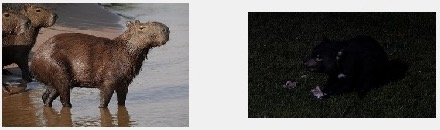
\includegraphics[scale=0.5]{imgs/failed-tc-hist.jpg}
    }
    \vspace{1cm}
    \subfloat[BoF with rbf SVM(上:ネガティブ判定された画像 下:ポジティブ判定された画像)]{
      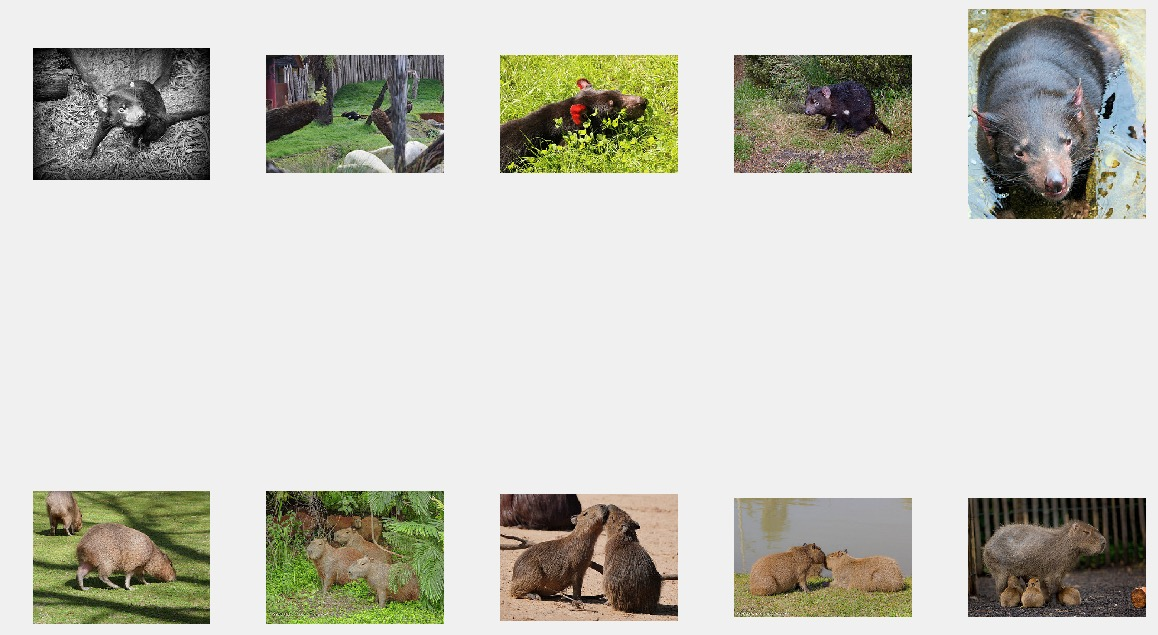
\includegraphics[scale=0.25]{imgs/failed-tc-bof.jpg}
    }
    \vspace{1cm}
    \subfloat[DCNN with linear SVM(bと同様)]{
      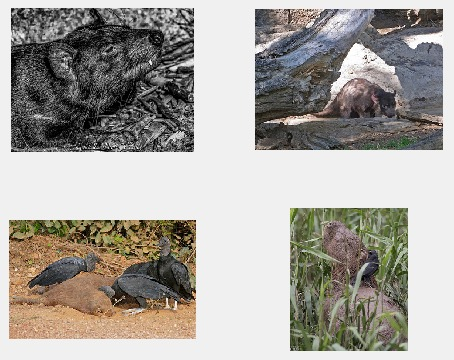
\includegraphics[scale=0.5]{imgs/failed-tc-dcnn.jpg}
    }
    \caption{t/b誤答画像一覧}
    \label{fig:tc}
  \end{center}
\end{figure}

\begin{figure}[t]
  \begin{center}
    \subfloat[Color histgram(左:判定対象画像 右:最近傍画像)]{
      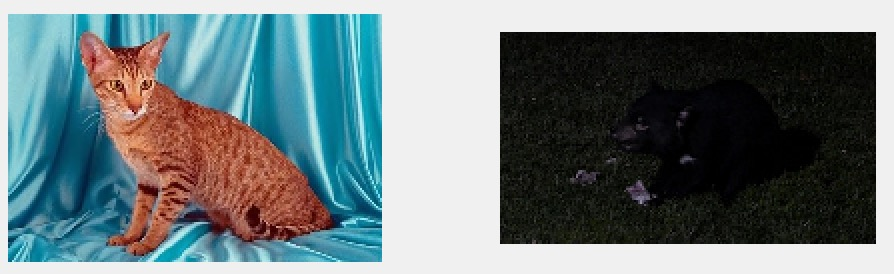
\includegraphics[scale=0.25]{imgs/failed-other-hist.jpg}
    }
    \vspace{1cm}
    \subfloat[BoF with rbf SVM(上:ネガティブ判定された画像 下:ポジティブ判定された画像)]{
      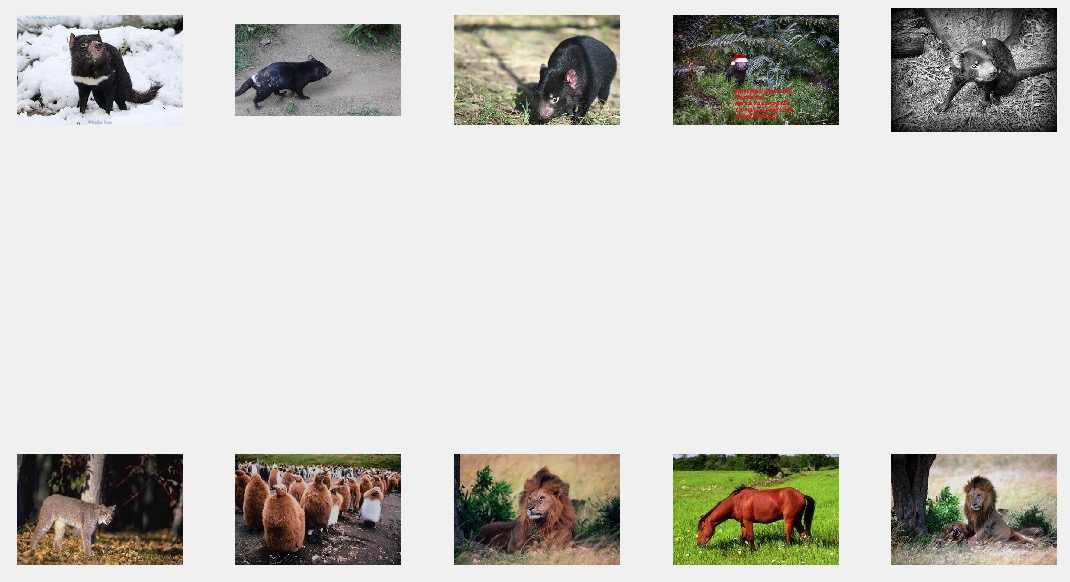
\includegraphics[scale=0.4]{imgs/failed-other-bof.jpg}
    }
    \vspace{1cm}
    \subfloat[DCNN with linear SVM(bと同様)]{
      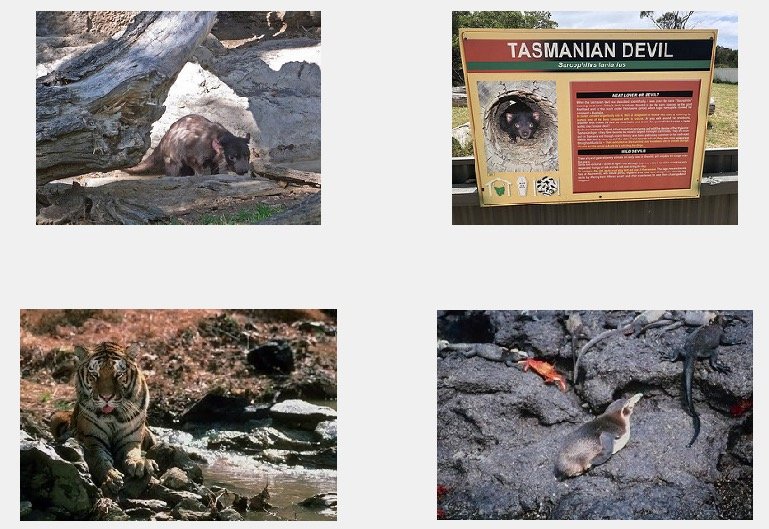
\includegraphics[scale=0.3]{imgs/failed-other-dcnn.jpg}
    }
    \caption{other誤答画像一覧}
    \label{fig:other}
  \end{center}
\end{figure}
\section{考察}
\subparagraph{カラーヒストグラムと最近傍分類}
3方法の中では、カラーヒストグラムが最も不安定な分類を行っていたことが読み取れた。
また、図\ref{fig:tc}, \ref{fig:other}
のカラーヒストグラムによる誤答画像を肉眼で見ても、
あまり類似性を見ることができなかった。
これはカラーヒストグラムによる最近傍分類は、
あまり精度の高いものではないことを強く示していると考えられた。

\subparagraph{BoFベクトルと非線形SVMによる分類}
t/c, other双方の適合率を見ると、カラーヒストグラムよりはいずれも高かった。
特にt/cにおいてはDCNNと比べても遜色ない精度となっていたものの、
otherにおいては明らかに精度が落ちていることが表\ref{tb:accuracy}から読み取れた。

これは、t/cにおいてはポジティブ/ネガティブ共に特定の種類の動物に限定していたたことにより、
分離平面を定めることが容易であったものの、otherではネガティブが特定の動物に限定していなかった
影響で分離が難しくなったことが原因として考えられる。

\subparagraph{MatConvnetの標準ネットワークによる DCNN特徴量と線形SVM}
t/c, otherともに適合率が約98\%と非常に安定した数値となっていた。

詳しく見るとotherの適合率がt/cより0.75\%優れた結果となっているが、
これはotherの全体のサンプル数がt/cの二倍であったことが影響していると考えられる。
\section{感想}
3種の画像認識による分類方法を実践することで、三者の認識方法の違いを知ることができた。
\chapter{Web画像検索リランキング実験}
\section{課題内容}
ポジティブ300枚(ノイズ有)とネガティブ900枚の画像データセットを対象に2クラス画像分類を行った。
今回対象としたのは以下のパターンである。
\begin{itemize}
  \item ポジティブ: タスマニアデビル
  \item ネガティブ: それ以外
\end{itemize}
なお"それ以外"とは、\texttt{/usr/local/class/object/bgimg}
に存在する900枚全ての画像を指す。
学習用の画像はポジティブ300枚から25 or 50枚と全ネガティブ画像を対象とし、
評価用の画像は残りのポジティブ画像とした。
学習方法はは、DCNN特徴量をMatConvNetで抽出して線形SVMを使用した。

最終的にポジティブ画像のソートなしの上位100枚中と、
SVMの出力スコア上位100枚中の正解率(ノイズは不正解)の比較を行った。
\section{設計方針}
\section{プログラムの説明}
\section{実験}
\section{考察}
\section{感想}

\appendix
\chapter{プログラムリスト}
\section{レポート課題1}
\subsection{codebook/filelist作成}
\lstinputlisting[caption=flist_thisdir.m]{src/report1/t.devil-capybara/histgram/flist\string_thisdir.m}
\lstinputlisting[caption=flist_others.m]{src/report1/t.devil-others/histgram/flist\string_others.m}
\lstinputlisting[caption=mk_codebook_tc.m]{src/report1/t.devil-capybara/histgram/mk\string_codebook\string_tc.m}
\lstinputlisting[caption=mk_codebook_other.m]{src/report1/t.devil-others/histgram/mk\string_codebook\string_other.m}
\subsection{カラーヒストグラムと最近傍分類}
\lstinputlisting[caption=capybara_hist.m]{src/report1/t.devil-capybara/histgram/capybara\string_hist.m}
\lstinputlisting[caption=others_hist.m]{src/report1/t.devil-others/histgram/others\string_hist.m}
\lstinputlisting[caption=mk_hist.m]{src/report1/t.devil-capybara/histgram/mk\string_hist.m}
\subsection{BoFベクトルと非線形SVMによる分類}
\lstinputlisting[caption=mk_code.m]{src/report1/t.devil-capybara/bof-svm/mk\string_code.m}
\lstinputlisting[caption=mk_code_other.m]{src/report1/t.devil-others/bof-svm/mk\string_code\string_others.m}
\lstinputlisting[caption=bof_svm_tc.m]{src/report1/t.devil-capybara/bof-svm/bof\string_svm\string_tc.m}
\lstinputlisting[caption=bof_svm_other.m]{src/report1/t.devil-others/bof-svm/bof\string_svm\string_others.m}
\subsection{MatConvnetの標準ネットワークによる DCNN特徴量と線形SVM}
\lstinputlisting[caption=mk_dcnnlist.m]{src/report1/t.devil-capybara/dcnn-svm/mk\string_dcnnlist.m}
\lstinputlisting[caption=dcnn_svm_tc.m]{src/report1/t.devil-capybara/dcnn-svm/dcnn\string_svm\string_tc.m}
\lstinputlisting[caption=dcnn_svm_other.m]{src/report1/t.devil-others/dcnn-svm/dcnn\string_svm\string_others.m}
\section{レポート課題2}
\lstinputlisting[caption=report2.m]{src/report2/report2.m}
\begin{thebibliography}{数字}
  \bibitem{key1} K.Yanai, "物体認識論 演習 レポート課題", the-UEC(Last modified: 27-Jan-2018)
\end{thebibliography}
\end{document}
